\documentclass[conference]{IEEEtran}
\pagestyle{plain}
\usepackage[pdftex]{graphicx}
\graphicspath{{../pdf/}{../jpeg/}}
\DeclareGraphicsExtensions{.pdf,.jpeg,.png}
\usepackage{changepage}
\usepackage[utf8]{inputenc}
\usepackage[T1]{fontenc}
\usepackage{matlab-prettifier}
\usepackage{circuitikz, siunitx}
\usepackage[cmex10]{amsmath}
\usepackage{mathabx}
\usepackage{algorithmic}
\usepackage{float}
\usepackage{array}
\usepackage{mdwmath}
\usepackage{mdwtab}
\usepackage{eqparbox}
\usepackage{url}
\usepackage{makecell}
\usepackage{tikz}
\usepackage{xcolor}
\usepackage{pgfplots}
\usepackage{booktabs}
\usepackage{subcaption}
\usepackage[backend=biber, style=ieee]{biblatex}
\addbibresource{biblio_traps_dynamics.bib}
\IEEEoverridecommandlockouts{}
\IEEEpeerreviewmaketitle{}

\pgfplotsset{compat=1.18} 
\usetikzlibrary{shapes.geometric, arrows, arrows.meta, positioning, patterns}

\tikzstyle{startstop} = [rectangle, rounded corners, 
minimum width=3cm, 
minimum height=1cm,
text centered, 
draw=black]

\tikzstyle{io} = [trapezium, 
trapezium stretches=true,
trapezium left angle=70, 
trapezium right angle=110, 
minimum width=3cm, 
minimum height=1cm, text centered, 
draw=black]

\tikzstyle{process} = [rectangle, 
minimum width=3cm, 
minimum height=1cm, 
text centered, 
text width=3cm, 
draw=black]

\tikzstyle{decision} = [diamond, 
minimum width=3cm, 
minimum height=1cm, 
text centered, 
draw=black]

\tikzstyle{arrow} = [thick,->,>=stealth,draw=black]
\tikzstyle{invarrow} = [thick,<-,>=stealth,draw=black]

\begin{document}

\title{Caracterización Estática y Análisis de Redes de Polarización en el JFET 2N5457 mediante Adquisición Automatizada de Datos}

\author{
    \authorblockN{
        B. Castro [1], A. Machado [2], L. Pineda [3], M. Rodríguez [4], J. Romero [5]
    }
    \authorblockA{
        \textit{Universidad de los Llanos} \\
        \textit{Villavicencio, Colombia} \\
        \begin{tabular}{c}
            \small \texttt{[1] 161004905 --- bacastro@unillanos.edu.co}            \\
            \small \texttt{[2] 161004922 --- ammachado@unillanos.edu.co}           \\
            \small \texttt{[3] 161004933 --- lapineda.sibo@unillanos.edu.co}       \\
            \small \texttt{[4] 161004834 --- marodriguez.payares@unillanos.edu.co} \\
            \small \texttt{[5] 161004937 --- jfromero.esquivel@unillanos.edu.co}   \\
        \end{tabular}
    }
}

\IEEEaftertitletext{\vspace{-1\baselineskip}}
\maketitle

% --- RESUMEN (ABSTRACT) ---
\begin{abstract}
    Este documento presenta la caracterización estática y el análisis comparativo de las redes de polarización fija (\textit{fixed-bias}), auto-polarización (\textit{self-bias}) y divisor de voltaje para el transistor de efecto de campo de unión (JFET) de canal n 2N5457. Mediante una metodología de instrumentación automatizada basada en un microcontrolador y scripts de procesamiento en Python, se adquirieron las familias de curvas características y se extrajeron los parámetros intrínsecos del dispositivo utilizando un algoritmo de ajuste por mínimos cuadrados. El software de optimización determinó una resistencia dinámica de salida en saturación $r_d \approx 5.99\,\text{k}\Omega$ y un parámetro de modulación de longitud de canal $\lambda \approx 0.026050\,\text{V}^{-1}$, evidenciando desviaciones sistemáticas respecto al modelo analítico ideal de Shockley. En los ensayos experimentales, la red \textit{fixed-bias} operó de forma persistente en la región de corte ($I_D = 0\,\text{mA}$) debido a que el voltaje aplicado ($V_{GS} = -1.451\,\text{V}$) superó el umbral absoluto de estrangulamiento o \textit{pinch-off}. Por el contrario, las configuraciones dotadas de lazos de retroalimentación en la fuente (\textit{self-bias} y divisor de voltaje) exhibieron una elevada estabilidad predictiva frente a las no idealidades del transistor. Los resultados convalidan la necesidad de incorporar los efectos físicos de segundo orden en el modelado matemático estático para el diseño robusto de etapas de amplificación de pequeña señal.
\end{abstract}

% --- PALABRAS CLAVE (KEYWORDS) ---
\begin{IEEEkeywords}
    Adquisición de datos, Ajuste de curvas, JFET 2N5457, Modulación de longitud de canal, Puntos de operación ($Q$), Redes de polarización.
\end{IEEEkeywords}
\section{Introducción}

El transistor de efecto de campo de unión (JFET) de canal n es un dispositivo
semiconductor fundamental controlado por voltaje, cuya operación se basa en la
modulación de la conductividad de su canal mediante el control de la región de
agotamiento, la cual es dictada por el voltaje puerta-fuente
(Fig.~\ref{fig:estructura_jfet}) ($V_{GS}$)~\cite{boylestad_dispositivos}. En
la presente práctica de laboratorio, el objeto de estudio es el modelo
comercial 2N5457, un dispositivo ampliamente utilizado en etapas de
amplificación de pequeña señal y conmutación analógica debido a sus
características de alta impedancia de entrada.

\begin{figure}[htbp]
    \centering
    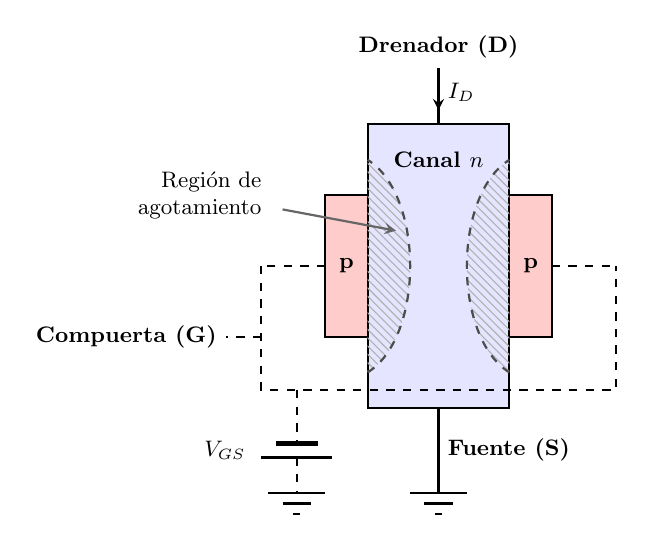
\begin{tikzpicture}[font=\small, >=stealth, scale=0.9, transform shape]
        % Canal N (Cuerpo principal)
        \draw[fill=blue!10, thick] (0,0) rectangle (2,4);
        \node at (1,3.5) {\textbf{Canal $n$}};

        % Zonas P (Terminales de la compuerta)
        \draw[fill=red!20, thick] (-0.6, 1) rectangle (0, 3);
        \draw[fill=red!20, thick] (2, 1) rectangle (2.6, 3);
        \node at (-0.3, 2) {\textbf{p}};
        \node at (2.3, 2) {\textbf{p}};

        % Regiones de Agotamiento (Depletion Regions) controladas por V_GS
        \draw[pattern=north west lines, pattern color=gray!60, draw=none]
        (0, 0.5) .. controls (0.8, 1) and (0.8, 3) .. (0, 3.5) -- cycle;
        \draw[pattern=north west lines, pattern color=gray!60, draw=none]
        (2, 0.5) .. controls (1.2, 1) and (1.2, 3) .. (2, 3.5) -- cycle;

        % Contornos punteados de las regiones de agotamiento para mayor claridad visual
        \draw[thick, dashed, color=black!70] (0, 0.5) .. controls (0.8, 1) and (0.8, 3) .. (0, 3.5);
        \draw[thick, dashed, color=black!70] (2, 0.5) .. controls (1.2, 1) and (1.2, 3) .. (2, 3.5);

        % Terminal Drenador (D) y dirección de corriente
        \draw[thick] (1,4) -- (1,4.8) node[above] {\textbf{Drenador (D)}};
        \draw[thick, ->] (1,4.7) -- (1,4.2) node[midway, right] {$I_D$};

        % Conexiones de la Compuerta (G) unidas en una sola terminal (trazo punteado)
        \draw[thick, dashed] (-0.6, 2) -- (-1.5, 2);
        \draw[thick, dashed] (2.6, 2) -- (3.5, 2);
        \draw[thick, dashed] (-1.5, 2) -- (-1.5, 0.25) -- (3.5, 0.25) -- (3.5, 2);
        \draw[thick, dashed] (-1.5, 1) -- (-2, 1) node[left, font=\small\bfseries, solid] {Compuerta (G)};

        % Fuente de voltaje V_GS referenciada a tierra (Terminal Negativa hacia Gate)
        \draw[thick, dashed] (-1, 0.25) -- (-1, -0.5);
        \draw[line width=2pt] (-1.3, -0.5) -- (-0.7, -0.5); % Placa negativa (corta/gruesa)
        \draw[thick] (-1.5, -0.7) -- (-0.5, -0.7);          % Placa positiva (larga/delgada)
        \node[left, font=\small] at (-1.6, -0.6) {$V_{GS}$};
        \draw[thick, dashed] (-1, -0.7) -- (-1, -1.2);

        % Símbolo de Tierra para V_GS
        \draw[thick] (-1.4, -1.2) -- (-0.6, -1.2);
        \draw[thick] (-1.2, -1.35) -- (-0.8, -1.35);
        \draw[thick] (-1.05, -1.5) -- (-0.95, -1.5);

        % Terminal Fuente (S) y su conexión a Tierra
        \draw[thick] (1,0) -- (1,-0.6) node[right] {\textbf{Fuente (S)}};
        \draw[thick] (1,-0.6) -- (1,-1.2);

        % Símbolo de Tierra para la Fuente (S)
        \draw[thick] (0.6, -1.2) -- (1.4, -1.2);
        \draw[thick] (0.8, -1.35) -- (1.2, -1.35);
        \draw[thick] (0.95, -1.5) -- (1.05, -1.5);

        % Etiqueta descriptiva apuntando a la región de depletación
        \node[text width=3cm, align=right] at (-3, 3) {Región de\\agotamiento};
        \draw[->, thick, color=gray!80!black] (-1.2, 2.8) -- (0.4, 2.5);

    \end{tikzpicture}
    \caption{Representación transversal geométrica de un JFET de canal n.}\label{fig:estructura_jfet}
\end{figure}

El análisis teórico clásico de polarización para estos transistores se
fundamenta en el modelo ideal descrito por la ecuación de Shockley, la cual
asume una resistencia de salida infinita ($r_d = \infty$) una vez el
dispositivo ingresa a la zona de saturación. No obstante, en componentes reales
como el 2N5457, se manifiesta de forma evidente el fenómeno de modulación de
longitud de canal, un comportamiento físico análogo al efecto Early en los
transistores de unión bipolar (BJT)~\cite{neamen_fisica_semiconductores}. Este
efecto de segundo orden produce una pendiente visible en las curvas
características de salida (Fig.~\ref{fig:ideal_vs_real_jfet}), generando una
fuga resistiva intrínseca que introduce discrepancias inevitables entre los
cálculos matemáticos de diseño ideal y las mediciones empíricas realizadas
sobre la protoboard.

El comportamiento eléctrico del transistor de efecto de campo de unión (JFET)
de canal n en su región de saturación se encuentra gobernado por sus
características físicas e intrínsecas de fabricación. La relación de
transferencia de naturaleza cuadrática, que vincula la corriente de drenador
con el voltaje de control compuerta-fuente, se modela analíticamente mediante
la ecuación de Shockley, expresada en~\eqref{eq:shockley}. Esta formulación
matemática constituye el pilar fundamental para el análisis predictivo, el uso
del método gráfico y el diseño asistido por computador de las redes de
polarización evaluadas en esta práctica:

\begin{equation}
    \label{eq:shockley}
    I_{D}=I_{DSS}{\left(1-\frac{V_{GS}}{V_{P}}\right)}^{2}
\end{equation}

\begin{figure}[htbp]
    \centering
    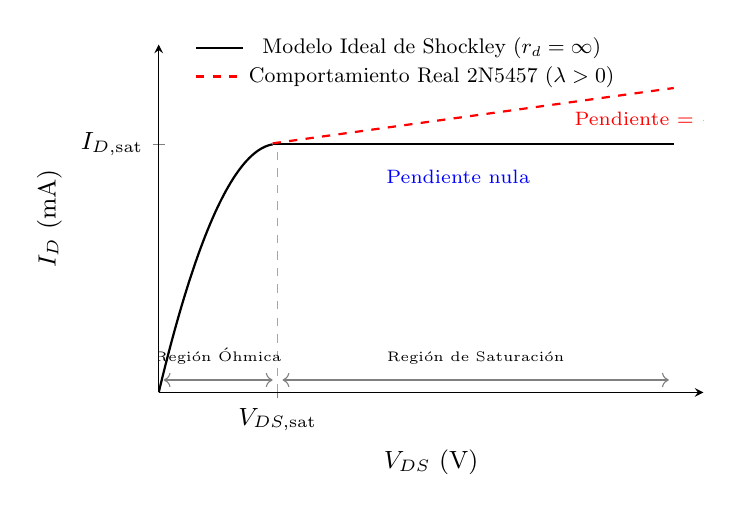
\begin{tikzpicture}
        \begin{axis}[
                axis lines = left,
                xlabel = {$V_{DS}$ (V)},
                ylabel = {$I_D$ (mA)},
                xmin = 0, xmax = 5.5,
                ymin = 0, ymax = 2.8,
                xtick = {1.2},
                xticklabels = {$V_{DS,\text{sat}}$},
                ytick = {2.0},
                yticklabels = {$I_{D,\text{sat}}$},
                font = \small,
                % Se ajusta la posición de la leyenda para evitar superposiciones
                legend style = {at={(0.05,1.05)}, anchor=north west, draw=none, fill=none,
                        nodes={scale=0.85, transform shape}}, width = 8.5cm, height = 6cm, grid = none
            ]

            % Definición explícita de los estilos en la leyenda sin la clave 'linear'
            \addlegendimage{black, thick}
            \addlegendentry{Modelo Ideal de Shockley ($r_d = \infty$)}
            \addlegendimage{red, dashed, thick}
            \addlegendentry{Comportamiento Real 2N5457 ($\lambda > 0$)}

            % 1. Región Óhmica o de Triodo (Común e idealizada continua hasta V_DS,sat)
            \addplot [domain=0:1.15, samples=50, thick, color=black] {2.0*(1 - (1 - x/1.2)^2)};

            % 2. Curva de Saturación - Modelo Ideal de Shockley (Línea azul continua horizontal)
            \addplot [domain=1.15:5.2, samples=2, thick, color=black] {2.0};

            % 3. Curva de Saturación - Comportamiento Real (Línea ROJA INTERLINEADA/DASHED con pendiente)
            \addplot [domain=1.15:5.2, samples=2, thick, color=red, dashed] {2.01 + 0.11*(x - 1.2)};

            % Línea de demarcación vertical discontinua para V_DS,sat
            \draw [dashed, color=gray!70] (axis cs:1.2,0) -- (axis cs:1.2,2.0);

            % Anotaciones vectoriales de las pendientes corregidas en posición
            \node [anchor=south west, color=blue] at (axis cs:2.2, 1.6) {\scriptsize Pendiente nula};
            \node [anchor=south west, color=red] at (axis cs:4.1, 1.98) {\scriptsize Pendiente $= \frac{1}{r_d}$};

            % Indicadores y delimitación de las zonas de operación
            \node [anchor=south] at (axis cs:0.6, 0.15) {\tiny Región Óhmica};
            \node [anchor=south] at (axis cs:3.2, 0.15) {\tiny Región de Saturación};
            \draw [style={<->}, color=gray] (axis cs:0.05, 0.1) -- (axis cs:1.15, 0.1);
            \draw [style={<->}, color=gray] (axis cs:1.25, 0.1) -- (axis cs:5.15, 0.1);
        \end{axis}
    \end{tikzpicture}
    \caption{Comparativa geométrica entre la curva de salida idealizada por la ecuación de Shockley y la respuesta real de un JFET.}\label{fig:ideal_vs_real_jfet}
\end{figure}

Para caracterizar adecuadamente el dispositivo y mitigar los errores
sistemáticos asociados a la toma manual de datos, se diseñó e implementó un
sistema automatizado de adquisición de alta resolución. El ecosistema de
hardware y software desarrollado integra un microcontrolador operado mediante
el firmware \texttt{captura.ino}, encargado de la digitalización precisa de las
señales analógicas. Posteriormente, la información es transmitida a un entorno
de procesamiento automatizado en Python conformado por los scripts
\texttt{captura.py} y \texttt{main.py}; dichas herramientas gestionan el
almacenamiento masivo, el filtrado de ruido y el ajuste de curvas
experimentales mediante algoritmos de mínimos cuadrados, permitiendo extraer
con alta fidelidad parámetros críticos del modelo matemático como el voltaje de
estrangulamiento ($V_p$) y la corriente de saturación de drenaje
($I_{DSS}$)~\cite{dunn_instrumentacion}.

El objetivo principal de este informe es caracterizar exhaustivamente el JFET
2N5457 y evaluar su desempeño bajo tres redes de polarización fundamentales
establecidas en la guía metodológica: polarización fija (\textit{fixed-bias},
Fig.~\ref{fig:fixed_bias}), autopolarización (\textit{self-bias},
Fig.~\ref{fig:self_bias}) y polarización por divisor de voltaje
(\textit{voltage-divider-bias}, Fig.~\ref{fig:voltage_divider_bias}). En las
siguientes secciones, el documento presenta de manera secuencial el análisis
metodológico de las curvas características extraídas, una comparación
cuantitativa entre los puntos de operación ($Q$) teóricos y los medidos
experimentalmente, y una discusión detallada sobre el impacto directo de las no
idealidades del dispositivo en la estabilidad de los circuitos implementados.

\begin{figure}[htbp]
    \centering
    \begin{circuitikz}[scale=0.7, transform shape, american voltages]
        % Transistor JFET de canal n
        \node[njfet] (J) at (0,0) {};

        % Malla de Drenaje (Drain): Corriente ID y Voltaje VD
        \draw (0, 4) node[circ] {} node[above] {$V_{DD}$} to[R, l=$R_D$, i=$I_D$] (J.D);
        \draw (J.D) node[circ] {} node[right] {$V_D$};

        % Malla de Surtidor (Source): Corriente IS
        \draw (J.S)  node[circ] {} node[right] {$V_S$} to[short, i=$I_S$] ++(0,-1.5) node[ground] {};

        % Malla de Compuerta (Gate): Corriente IG y Voltaje VG
        \draw (J.G) node[circ] {} node[above] {$V_G$} ++(0,0) coordinate(G_conn);

        % Resistencia RG y Fuente VGG
        \draw (G_conn) to[short, i<_=$I_G$] ++(-2,0) to[V, l_=$V_{GG}$, invert] ++(0,-2) node[ground] {};

    \end{circuitikz}
    \caption{Red de polarización fija (\textit{Fixed-Bias}) para el transistor JFET de canal n 2N5457.}\label{fig:fixed_bias}
\end{figure}

\begin{figure}[htbp]
    \centering
    \begin{circuitikz}[scale=0.7, transform shape, american voltages]
        % Transistor JFET de canal n
        \node[njfet] (J) at (0,0) {};

        % Malla de Drenaje (Drain): Corriente ID y Voltaje VD
        \draw (0, 4) node[circ] {} node[above] {$V_{DD}$} to[R, l=$R_D$, i>=$I_D$] (J.D);
        \draw (J.D) node[circ] {} node[right=2pt] {$V_D$};

        % Malla de Surtidor (Source): Corriente IS a través de RS
        \draw (J.S)  node[circ] {} node[right] {$V_S$} to[R, l=$R_S$, i=$I_S$] ++(0,-2.5) node[ground] {};

        % Malla de Compuerta (Gate): Corriente IG y Voltaje VG
        \draw (J.G) node[circ] {} node[above] {$V_G$} to[short, i<=$I_G$] ++(-2,0) to[short] ++(0,-3) node[ground] {};

    \end{circuitikz}
    \caption{Red de autopolarización (\textit{Self-Bias}) para el transistor JFET de canal n 2N5457.}\label{fig:self_bias}
\end{figure}

\begin{figure}[htbp]
    \centering
    \begin{circuitikz}[scale=0.7, transform shape, american voltages]
        % Transistor JFET de canal n
        \node[njfet] (J) at (0,0) {};

        % Rama Derecha: Drain (ID, VD) y Source (IS)
        \draw (J.D)  node[circ] {} node[right] {$V_D$} to[R, l_=$R_D$, i<=$I_D$] ++ (0, 3.0) coordinate(top_right) to[short] ++(0,1) node[circ] {} node[above] {$V_{DD}$};
        \draw (top_right) to[short] ++(-2.5,0) to[R, l_=$R_1$] ++(0,-3.0) to[short] ++(0,-1.05) coordinate(divisor) to[short, i>=$I_G$] (J.G) node[circ] {} node[above] {$V_{G}$};
        \draw (divisor) to[R, l_=$R_2$] ++(0,-3.5) node[ground] {};
        \draw (J.S) node[circ] {} node[right] {$V_S$} to[R, l=$R_S$, i=$I_S$] ++(0,-3.0) node[ground] {};

    \end{circuitikz}
    \caption{Red de polarización por divisor de voltaje (\textit{Voltage-Divider-Bias}) para el transistor JFET de canal n 2N5457.}\label{fig:voltage_divider_bias}
\end{figure}

Con el objetivo de asegurar la reproducibilidad de los experimentos y el
análisis de datos presentados, el conjunto completo de herramientas de software
desarrolladas para este laboratorio se encuentra disponible de forma pública.
Los scripts correspondientes al firmware de adquisición en el microcontrolador
(\texttt{captura.ino}), la interfaz de captura serial en Python
(\texttt{captura.py}) y el algoritmo de ajuste de curvas por mínimos cuadrados
para el cálculo de los parámetros del JFET (\texttt{main.py}) pueden ser
consultados y descargados en el repositorio público de GitHub:
\url{https://github.com/Nocudo/Lab-4}.

\section{Metodología Experimental y Computacional}
La metodología implementada para la caracterización y análisis del transistor
JFET 2N5457 se desarrolló de forma secuencial y cronológica, integrando
herramientas de instrumentación electrónica automatizada y entornos de cómputo
numérico. La estructura general del proceso se detalla en el diagrama de
bloques de la Fig.~\ref{fig:diagrama_bloques}.

\begin{figure}[htbp]
    \centering
    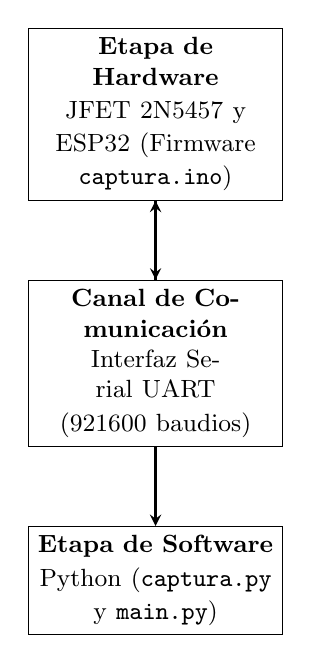
\begin{tikzpicture}[node distance=1cm, auto, >=latex']
        % Nodos distribuidos verticalmente
        \node [process] (hw) {\small \textbf{Etapa de Hardware}\\ JFET 2N5457 y ESP32 (Firmware \texttt{captura.ino})};
        \node [process, below= of hw] (serial) {\small \textbf{Canal de Comunicación}\\ Interfaz Serial UART \\ (921600 baudios)};
        \node [process, below= of serial] (sw) {\small \textbf{Etapa de Software}\\ Python (\texttt{captura.py} y \texttt{main.py})};

        % Conexiones verticales directas
        \path [arrow] (hw.south) -- (serial.north);
        \path [arrow] (serial.north) -- (hw.south); % Si requieres flujo bidireccional
        \path [arrow] (serial.south) -- (sw.north);
    \end{tikzpicture}
    \caption{Diagrama de bloques del ecosistema de adquisición automatizada y procesamiento de datos.}~\label{fig:diagrama_bloques}
\end{figure}

\subsection{Sistema de Adquisición Automatizado (Hardware y Software)}
En primera instancia, se diseñó e implementó un entorno tecnológico orientado a
la digitalización eficiente de variables eléctricas, con el propósito de
mitigar los errores de apreciación geométrica asociados a las lecturas de
instrumentos analógicos tradicionales. La infraestructura de hardware se
fundamentó en el uso de un microcontrolador programado mediante el firmware
\texttt{captura.ino}. Este dispositivo operó como un convertidor
analógico-digital (ADC) de alta velocidad, muestreando en tiempo real las
caídas de tensión en los nodos del transistor mediante sus canales de entrada
analógica y promediando las lecturas para atenuar componentes de ruido
electromagnético de alta frecuencia.

En la Figura 1 se presenta el esquema eléctrico del circuito de
acondicionamiento y adquisición de señal diseñado para el control y monitoreo
del transistor JFET\@. El sistema consta de una etapa inicial de amplificación
y desplazamiento basada en el amplificador operacional $U_1$ en configuración
inversora con una ganancia de tensión de $10$ ($R_3 = 100\text{ k}\Omega$ y
$R_1 = 10\text{ k}\Omega$). Esta etapa procesa una señal senoidal de entrada de
$2\text{ V}_{pp}$ a $1\text{ Hz}$ con un offset de $1\text{ V}$ para entregar
una señal de salida de $20\text{ V}_{pp}$ completamente positiva en el nodo
$V_a$. Posteriormente, este voltaje se acopla al terminal de drenaje del
transistor $Q_1$ a través de la resistencia limitadora $R_4 = 220\ \Omega$. Con
el fin de garantizar una adquisición de datos segura mediante los canales
analógicos del microcontrolador ESP32, se implementan dos divisores de tensión
idénticos en los nodos de medición $V_a$ y $V_b$ utilizando resistencias de
$4250\ \Omega$ (superior) y $750\ \Omega$ (inferior), adecuando el rango
dinámico de las señales al límite operativo del ADC\@.

\begin{figure}[htbp]
    \centering
    \begin{circuitikz}[scale=0.55, transform shape, american voltages]

        % --- ETAPA DE ENTRADA Y AMPLIFICACIÓN (OPAMP) ---
        % Amplificador Operacional U1
        \node[op amp] (U1) at (4, 3) {};
        \node[above=6pt] at (U1.north) {$U_1$};

        % Conexión de la entrada no inversora (+) a tierra
        \draw (U1.+) -- ++(0,-0.5) node[ground] {};

        % Nodo de suma en la entrada inversora (-)
        \draw (U1.-) -- ++(-1, 0) coordinate(junc) node[circ] {};

        % Rama de señal de entrada Vin (R2 y Fuente)
        \draw (junc) -- ++(0, 0) to[R, l=$R_2$, a_=10k$\Omega$] ++(-2.5, 0)
        to[sV, l=$V_{in}$] ++(0, -2.5) node[ground] {};

        % Lazo de realimentación (R3)
        \draw (junc) -- ++(0, 2.2) coordinate(fb_top)
            to[R, l=$R_3$, a=100k$\Omega$] (fb_top -| U1.out) -- (U1.out) node[circ] {};

        % --- ETAPA DEL TRANSISTOR JFET Y DIVISORES DE TENSIÓN ---
        % Nodo Va y resistencia de drenaje R4
        \draw (U1.out) -- ++(0.5, 0) node[circ] {} coordinate(Va_node) node[above right] {$V_a$}
            to[R, l=$R_4$, a=220$\Omega$] ++(4, 0) node[circ] {} coordinate(Vb_node) node[above left] {$V_b$};

        % Divisor de tensión A (Conectado al nodo Va)
        \draw (Va_node) to[R, l=$R_5$, a=4250$\Omega$] ++(0, -2.5) node[circ] {} coordinate(espA)
            to[R, l=$R_6$, a=750$\Omega$] ++(0, -2) node[ground] {};
        \draw (espA) to[short, -o] ++(0.5, 0) node[right] {\scriptsize ESP32\_Va};

        % Transistor JFET Q1 conectado al nodo Vb (Drain)
        \draw (Vb_node) to[short] ++(0, -0.5) node[njfet, anchor=D] (Q1){};
        \node[right] at (Q1.center) {$Q_1$};
        \draw (Q1.S) -- ++(0, -0.5) node[ground] {};
        \draw (Q1.G) to[short, -o] ++(-0.5, 0) node[left] {$V_{GS}$};

        % Divisor de tensión B (Conectado al nodo Vb extendido a la derecha)
        \draw (Vb_node) -- ++(2.5, 0) node[circ] {} coordinate(Vb_div)
            to[R, l=$R_7$, a=4250$\Omega$] ++(0, -2.5) node[circ] {} coordinate(espB)
            to[R, l=$R_8$, a=750$\Omega$] ++(0, -2) node[ground] {};
        \draw (espB) to[short, -o] ++(0.5, 0) node[right] {\scriptsize ESP32\_Vb};
    \end{circuitikz}
    \caption{Circuito detallado de acondicionamiento de señal y acoplamiento al transistor JFET con salidas para ADC.}\label{fig:circuito_acondicionamiento_completo}
\end{figure}

La automatización del proceso de caracterización se fundamenta en la co-diseño
de un ecosistema de hardware y software compuesto por dos bloques programables
independientes. En primer lugar, se desarrolló el firmware \texttt{captura.ino}
en lenguaje C++ para el microcontrolador ESP32, el cual actúa como una unidad
de adquisición de datos en tiempo real de alta velocidad encargada del muestreo
analógico de las señales del JFET\@. En segundo lugar, se implementó el script
de control superior \texttt{captura.py} en Python, el cual gestiona la
sincronización temporal, la apertura del canal de comunicación serial a alta
velocidad (\num{921600} baudios), la recepción estructurada de los flujos
analógicos digitalizados y su posterior almacenamiento en archivos planos
indexados con formato CSV\@. El flujo lógico y secuencial de ambos componentes
de software se detalla en los diagramas de las Figuras~\ref{fig:flow_ino}
y~\ref{fig:flow_py}.

\begin{figure*}[htbp]
    \centering
    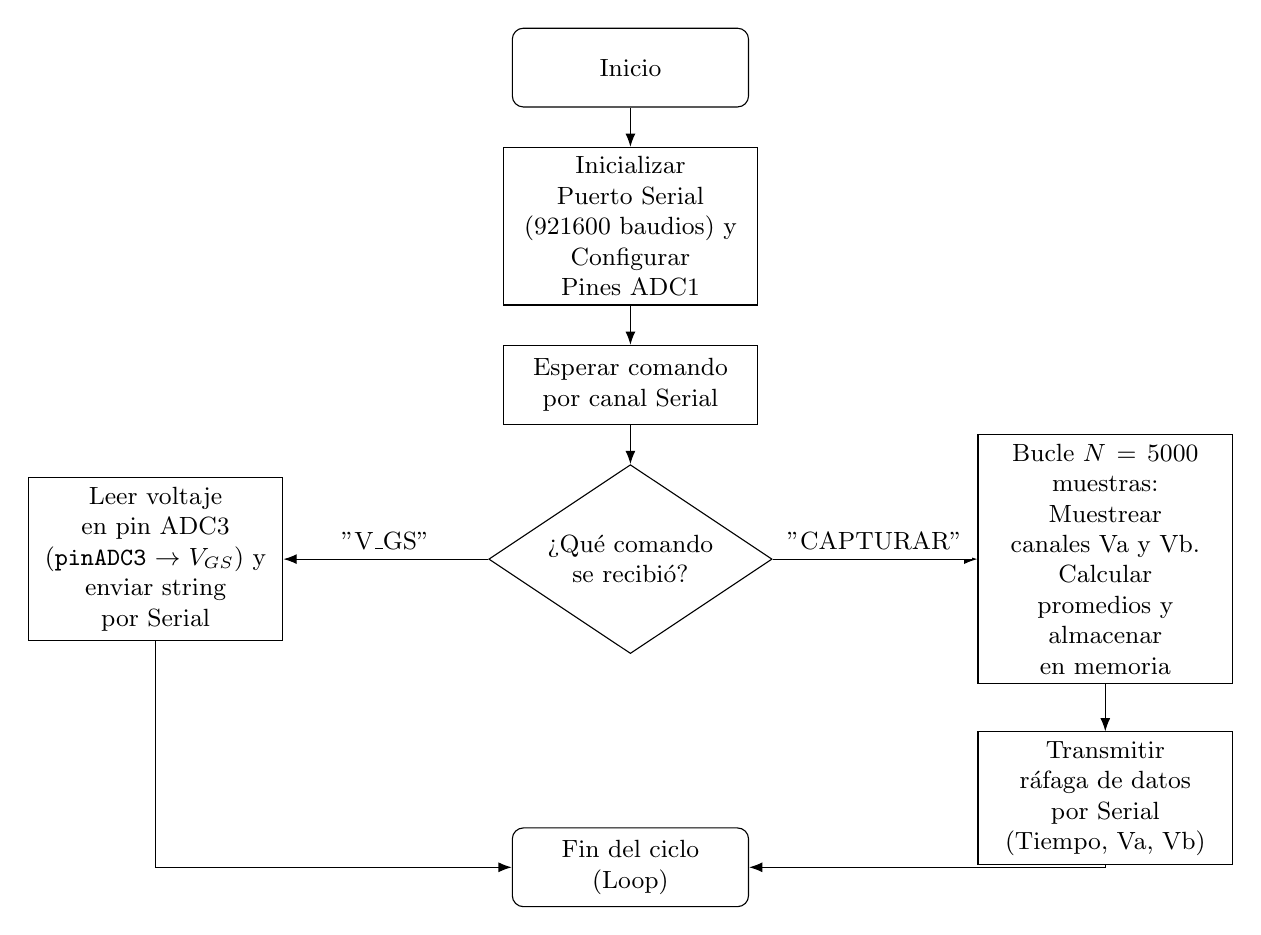
\begin{tikzpicture}[node distance=1.5cm, every node/.style={fill=white, font=\small}, align=center]

        % Nodos
        \node (start) [startstop] {Inicio};
        \node (init) [process, below=0.5cm of start] {Inicializar Puerto Serial\\(921600 baudios) y\\Configurar Pines ADC1};
        \node (wait) [process, below=0.5cm of init] {Esperar comando\\por canal Serial};
        \node (decide) [draw, diamond, aspect=1.5, below=0.5cm of wait] {¿Qué comando\\se recibió?};
        \node (vgs) [process, left=1.2cm of decide, xshift=-1.4cm] {Leer voltaje en pin ADC3\\(\texttt{pinADC3} $\rightarrow V_{GS}$) y\\enviar string por Serial};
        \node (cap) [process, right=1.2cm of decide, xshift=1.4cm] {Bucle $N=5000$ muestras:\\Muestrear canales Va y Vb.\\Calcular promedios y\\almacenar en memoria};
        \node (stream) [process, below=0.6cm of cap] {Transmitir ráfaga de datos\\por Serial\\(Tiempo, Va, Vb)};
        \node (end) [startstop, below=2.2cm of decide] {Fin del ciclo\\(Loop)};

        % Conexiones
        \draw [-{Latex}] (start) -- (init);
        \draw [-{Latex}] (init) -- (wait);
        \draw [-{Latex}] (wait) -- (decide);
        \draw [-{Latex}] (decide) -- node[above] {"V\_GS"} (vgs.east);
        \draw [-{Latex}] (decide) -- node[above] {"CAPTURAR"} (cap.west);
        \draw [-{Latex}] (cap) -- (stream);
        \draw [-{Latex}] (vgs) |- (end);
        \draw [-{Latex}] (stream) |- (end);

    \end{tikzpicture}
    \caption{Diagrama de flujo del firmware alojado en el microcontrolador (\texttt{captura.ino}).}\label{fig:flow_ino}
\end{figure*}

\begin{figure}[htbp]
    \centering
    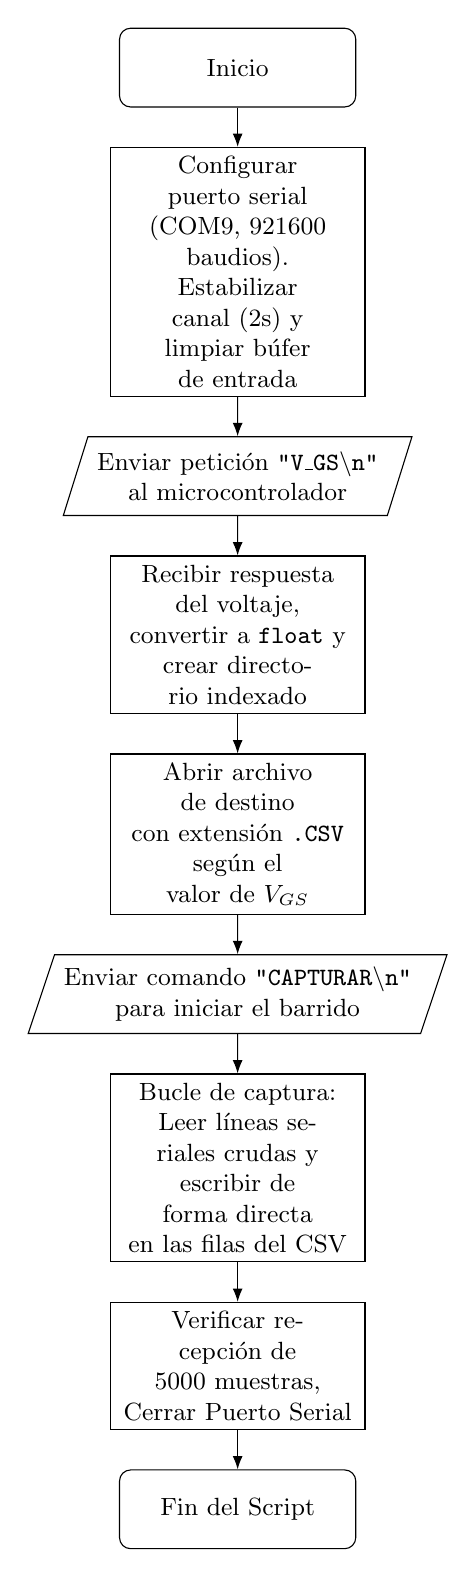
\begin{tikzpicture}[node distance=1.5cm, every node/.style={fill=white, font=\small}, align=center]

        % Nodos
        \node (start) [startstop] {Inicio};
        \node (init) [process, below=0.5cm of start] {Configurar puerto serial\\(COM9, 921600 baudios).\\Estabilizar canal (2s) y\\limpiar búfer de entrada};
        \node (req1) [io, below=0.5cm of init] {Enviar petición \texttt{"V\_GS\textbackslash n"}\\al microcontrolador};
        \node (read1) [process, below=0.5cm of req1] {Recibir respuesta del voltaje,\\convertir a \texttt{float} y\\crear directorio indexado};
        \node (file) [process, below=0.5cm of read1] {Abrir archivo de destino\\con extensión \texttt{.CSV}\\según el valor de $V_{GS}$};
        \node (req2) [io, below=0.5cm of file] {Enviar comando \texttt{"CAPTURAR\textbackslash n"}\\para iniciar el barrido};
        \node (loop) [process, below=0.5cm of req2] {Bucle de captura:\\Leer líneas seriales crudas y\\escribir de forma directa\\en las filas del CSV};
        \node (close) [process, below=0.5cm of loop] {Verificar recepción de\\$5000$ muestras,\\Cerrar Puerto Serial};
        \node (end) [startstop, below=0.5cm of close] {Fin del Script};

        % Conexiones
        \draw [-{Latex}] (start) -- (init);
        \draw [-{Latex}] (init) -- (req1);
        \draw [-{Latex}] (req1) -- (read1);
        \draw [-{Latex}] (read1) -- (file);
        \draw [-{Latex}] (file) -- (req2);
        \draw [-{Latex}] (req2) -- (loop);
        \draw [-{Latex}] (loop) -- (close);
        \draw [-{Latex}] (close) -- (end);

    \end{tikzpicture}
    \caption{Diagrama de flujo del script supervisor ejecutado en Python (\texttt{captura.py}).}\label{fig:flow_py}
\end{figure}

\subsection{Caracterización y Extracción de Parámetros del JFET 2N5457}
Una vez consolidado el sistema de adquisición, se procedió con la primera fase
experimental dictada por la guía metodológica, la cual se enfocó en el mapeo
empírico de las curvas de transferencia y de salida del dispositivo
semiconductor bajo estudio. Este programa actúa como el motor analítico del
laboratorio; en primer lugar, indexa y filtra los archivos \texttt{.CSV}
generados en la etapa de captura para eliminar ruidos de digitalización
mediante umbrales adaptativos. Posteriormente, ejecuta un algoritmo de
regresión no lineal basado en el método de mínimos cuadrados (\textit{curve
    fitting}) para ajustar las curvas experimentales a la ecuación de Shockley,
extrayendo con precisión estadística los parámetros intrínsecos $I_{DSS}$,
$V_p$, $\lambda$ y la resistencia de salida $r_d$. Con estas variables reales
calibradas, el script resuelve los sistemas de ecuaciones no lineales de las
tres mallas de polarización utilizando métodos numéricos de convergencia,
exportando las gráficas de las familias de curvas y consolidando el reporte
analítico en el archivo plano \texttt{resultados\_2N5457.txt}. La secuencia
lógica de este script se describe en la Figura~\ref{fig:flow_main}. El
procedimiento analítico se dividió en las siguientes fases cronológicas:
\begin{enumerate}
    \item \textbf{Curva de control inicial:} Se cortocircuitó la terminal de la compuerta con la fuente para fijar de manera estricta un voltaje puerta-fuente nulo ($V_{GS} = 0\,\text{V}$). Bajo esta condición, se ejecutó un barrido dinámico de voltaje drenador-fuente ($V_{DS}$) mientras se registraba el comportamiento de la corriente de drenador ($I_D$), permitiendo obtener una aproximación preliminar y visual del voltaje de estrangulamiento o \textit{pinch-off} ($V_p$).
    \item \textbf{Familias de curvas de salida:} Posteriormente, se varió de forma discreta y controlada el voltaje de control $V_{GS}$ en el rango operativo del transistor, adquiriendo aproximadamente 35 perfiles cinéticos diferentes. Este barrido multifactorial permitió modelar con alta densidad de puntos la transición geométrica entre la región óhmica (trioda) y la región de saturación (activa) del JFET\@.
    \item \textbf{Ajuste paramétrico computacional:} Los datos experimentales de las corrientes de saturación correspondientes a cada nivel de $V_{GS}$ fueron procesados mediante el algoritmo central del script \texttt{main.py}. Este software aplicó un procedimiento de regresión no lineal basado en el método de mínimos cuadrados ponderados sobre la ecuación clásica de Shockley:
\end{enumerate}

\begin{figure}[htbp]
    \centering
    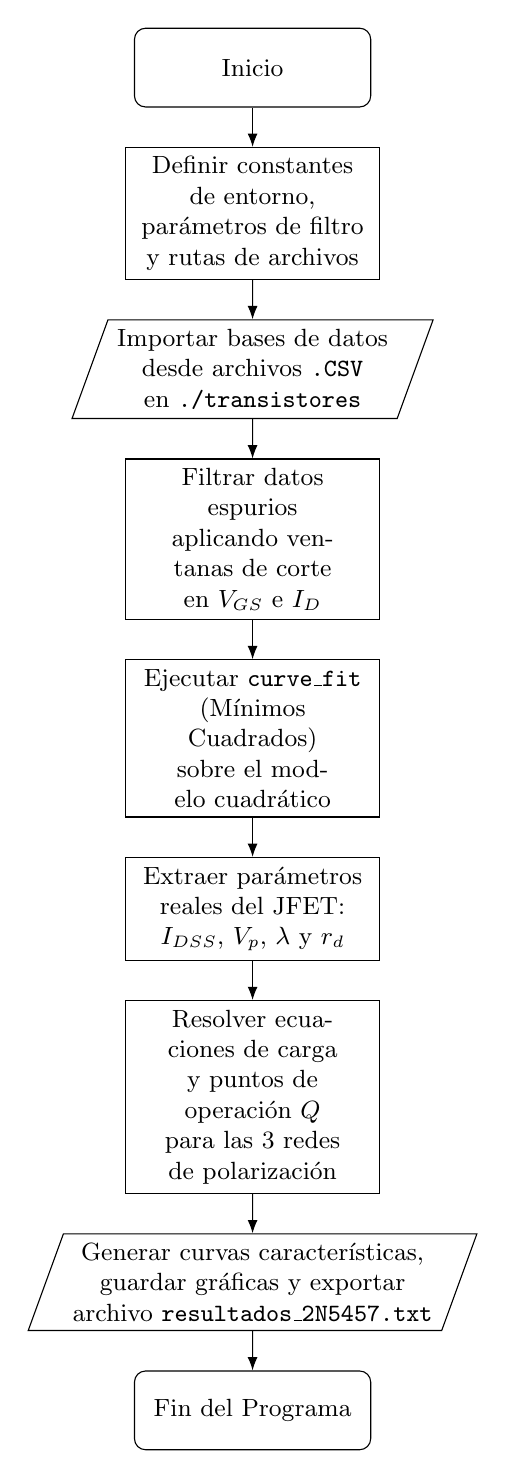
\begin{tikzpicture}[node distance=1.4cm, every node/.style={fill=white, font=\small}, align=center]

        % Nodos
        \node (start) [startstop] {Inicio};
        \node (init) [process, below=0.5cm of start] {Definir constantes de entorno,\\parámetros de filtro\\y rutas de archivos};
        \node (read) [io, below=0.5cm of init] {Importar bases de datos\\desde archivos \texttt{.CSV}\\en \texttt{./transistores}};
        \node (filter) [process, below=0.5cm of read] {Filtrar datos espurios\\aplicando ventanas de corte\\en $V_{GS}$ e $I_D$};
        \node (fit) [process, below=0.5cm of filter] {Ejecutar \texttt{curve\_fit}\\(Mínimos Cuadrados)\\sobre el modelo cuadrático};
        \node (extract) [process, below=0.5cm of fit] {Extraer parámetros reales del JFET:\\$I_{DSS}$, $V_p$, $\lambda$ y $r_d$};
        \node (solve) [process, below=0.5cm of extract] {Resolver ecuaciones de carga\\y puntos de operación $Q$\\para las 3 redes de polarización};
        \node (output) [io, below=0.5cm of solve] {Generar curvas características,\\guardar gráficas y exportar\\archivo \texttt{resultados\_2N5457.txt}};
        \node (end) [startstop, below=0.5cm of output] {Fin del Programa};

        % Conexiones
        \draw [-{Latex}] (start) -- (init);
        \draw [-{Latex}] (init) -- (read);
        \draw [-{Latex}] (read) -- (filter);
        \draw [-{Latex}] (filter) -- (fit);
        \draw [-{Latex}] (fit) -- (extract);
        \draw [-{Latex}] (extract) -- (solve);
        \draw [-{Latex}] (solve) -- (output);
        \draw [-{Latex}] (output) -- (end);

    \end{tikzpicture}
    \caption{Diagrama de flujo del algoritmo de procesamiento matemático, ajuste de curvas y resolución de redes de polarización (\texttt{main.py}).}\label{fig:flow_main}
\end{figure}

\subsection{Implementación y Medición de las Redes de Polarización}
En la fase final del desarrollo experimental, se diseñaron y ensamblaron sobre
una matriz de contactos (\textit{protoboard}) tres topologías de polarización
de corriente continua de uso común en ingeniería electrónica. El comportamiento
estático de cada red se evaluó alterando intencionalmente las condiciones de
carga pasiva para estudiar la estabilidad del punto de operación estático
($Q$):

\begin{itemize}
    \item \textbf{Configuración de Polarización Fija (\textit{Fixed-Bias}):} Se construyó la malla de entrada aplicando un voltaje de control constante en la compuerta. La respuesta del circuito se caracterizó bajo tres condiciones de carga lineal diferentes mediante la sustitución sucesiva de la resistencia de drenador ($R_D$).
    \item \textbf{Configuración de Autopolarización (\textit{Self-Bias}):} Se implementó la red realimentada por fuente y se evaluó dinámicamente mediante la variación sistemática de tres combinaciones complementarias de valores para la resistencia de drenador ($R_D$) y la resistencia de fuente ($R_S$).
    \item \textbf{Configuración de Polarización por Divisor de Voltaje (\textit{Voltage-Divider-Bias}):} Se estructuró una red de instrumentación robusta mediante un puente resistivo en la entrada. Para este circuito, se modificaron y analizaron tres conjuntos independientes de valores para el cuarteto resistivo constituido por $R_1$, $R_2$, $R_D$ y $R_S$.
\end{itemize}

Para cada una de las variaciones físicas efectuadas en los tres circuitos
anteriores, se recolectaron sistemáticamente las variables eléctricas puntuales
mediante instrumentos de medición digital calibrados. Los registros fueron
estructurados de forma automática dentro del archivo de texto plano
\texttt{resultados\_lab\_2N5457.txt}, discriminando las siguientes variables:
\begin{itemize}
    \item \textbf{Voltajes de nodo respecto a referencia:} Voltaje de drenador ($V_D$), voltaje de compuerta ($V_G$) y voltaje de fuente ($V_S$).
    \item \textbf{Corrientes de terminal:} Corriente de drenador ($I_D$), corriente de fuente ($I_S$) y corriente de compuerta ($I_G$).
\end{itemize}

Esta base de datos experimental se preservó de forma íntegra con el propósito
de efectuar, en las etapas posteriores del informe, un análisis comparativo y
de error relativo frente a las predicciones del modelo gráfico y las
simulaciones numéricas ideales de corriente continua.

\section{Análisis de Resultados e Interpretación Física}

Previo al análisis estático del dispositivo, el ecosistema de adquisición
automatizada registró las variables dinámicas en el dominio del tiempo para
validar la integridad de las señales analógicas digitalizadas por el ESP32. En
la Figura~\ref{fig:wave_voltaje} se exhibe el comportamiento temporal del
voltaje capturado a través de los canales del ADC, evidenciando la
sincronización y estabilidad del barrido automatizado. De forma complementaria,
la Figura~\ref{fig:wave_corriente} presenta el perfil de corriente transitoria
derivado de la caída de potencial en la resistencia de instrumentación,
confirmando la ausencia de componentes espurios significativos o ruidos de alta
frecuencia de gran amplitud antes del filtrado digital en Python.

\begin{figure}[htbp]
    \centering
    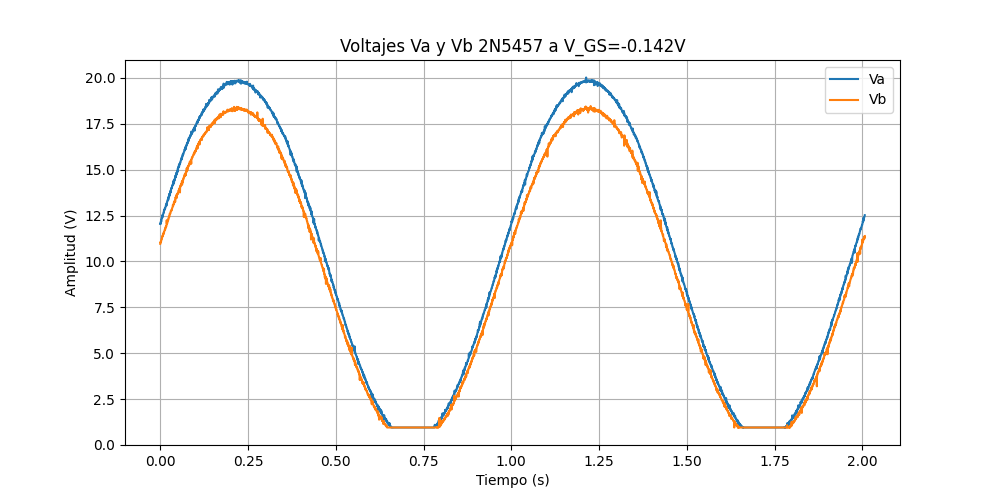
\includegraphics[width=\columnwidth]{voltaje.png}
    \caption{Señales temporales de voltaje capturadas por la etapa de instrumentación del sistema DAQ.}\label{fig:wave_voltaje}
\end{figure}

\begin{figure}[htbp]
    \centering
    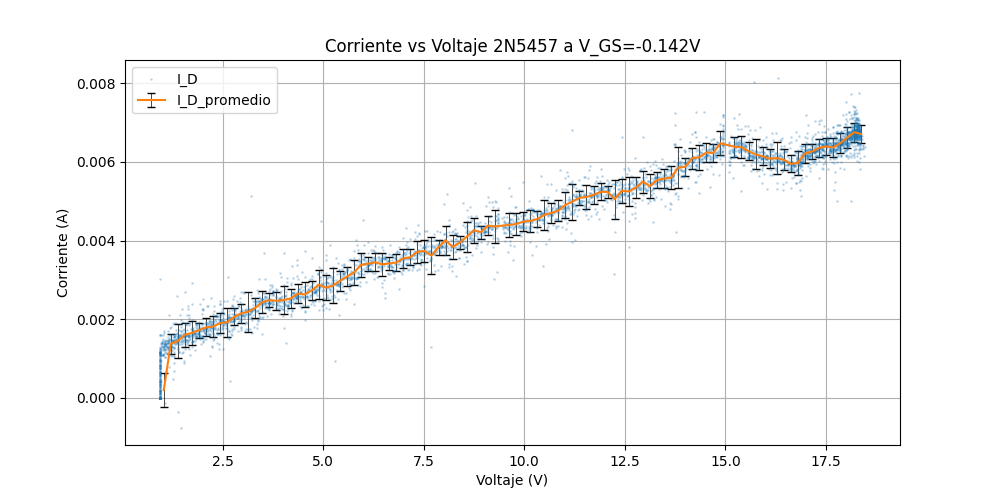
\includegraphics[width=\columnwidth]{corriente.png}
    \caption{Perfil de corriente en el dominio del tiempo registrado durante el barrido automatizado.}\label{fig:wave_corriente}
\end{figure}

Una vez consolidadas las bases de datos en formato de texto plano, el script
\texttt{main.py} ejecutó el análisis de regresión no lineal para remover las
desviaciones instrumentales y aislar el comportamiento intrínseco del
semiconductor. La Figura~\ref{fig:regresion_id} ilustra el proceso de
optimización matemática y ajuste por mínimos cuadrados aplicado sobre los
vectores de corriente filtrados, minimizando el error cuadrático medio frente a
las lecturas experimentales crudas.

Como resultado directo de esta optimización, la Figura~\ref{fig:curva_trans}
expone la curva de transferencia estática ($I_D$ vs. $V_{GS}$) del transistor
2N5457. En esta gráfica se contrasta la distribución de los puntos empíricos
medidos frente a la traza analítica calculada mediante el modelo calibrado de
Shockley, convalidando gráficamente la precisión del ajuste en la región de
saturación y permitiendo la localización matemática exacta del voltaje de corte
($V_p$) e $I_{DSS}$.

\begin{figure}[htbp]
    \centering
    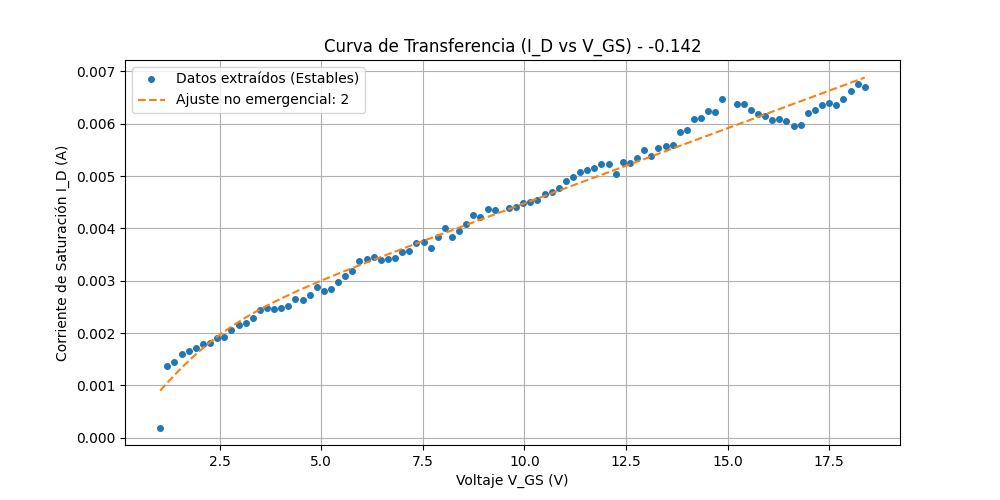
\includegraphics[width=\columnwidth]{regresion_corriente.png}
    \caption{Procesamiento estadístico y regresión numérica de los datos de corriente de drenador.}\label{fig:regresion_id}
\end{figure}

\begin{figure}[htbp]
    \centering
    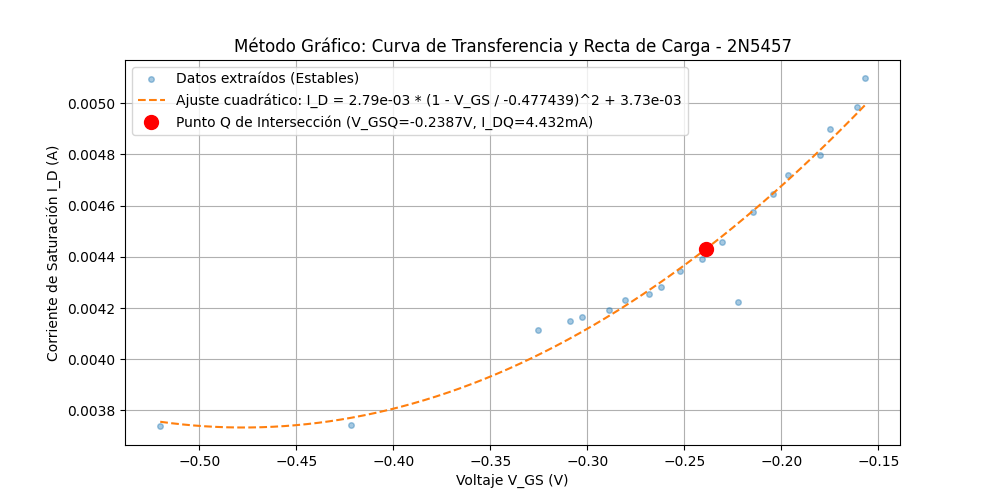
\includegraphics[width=\columnwidth]{curva_transferencia.png}
    \caption{Curva de transferencia experimental y modelo cuadrático ajustado de Shockley para el JFET 2N5457.}\label{fig:curva_trans}
\end{figure}

La consolidación final de la caracterización del dispositivo se presenta en la
Figura~\ref{fig:familia_curvas}, la cual despliega la familia de curvas
características de drenador ($I_D$ vs. $V_{DS}$) indexadas para los diferentes
pasos de voltaje de compuerta-fuente ($V_{GS}$) configurados de manera externa.
En este gráfico se aprecia con total claridad la transición del transistor
desde la región óhmica o de triodo hacia la región de saturación. Asimismo, la
pendiente incremental y sostenida que exhiben las trazas en la zona activa pone
de manifiesto el impacto del fenómeno físico de modulación de longitud de canal
($\lambda$), aportando el soporte gráfico que justifica las no idealidades
analizadas en los resultados de polarización.

\begin{figure}[htbp]
    \centering
    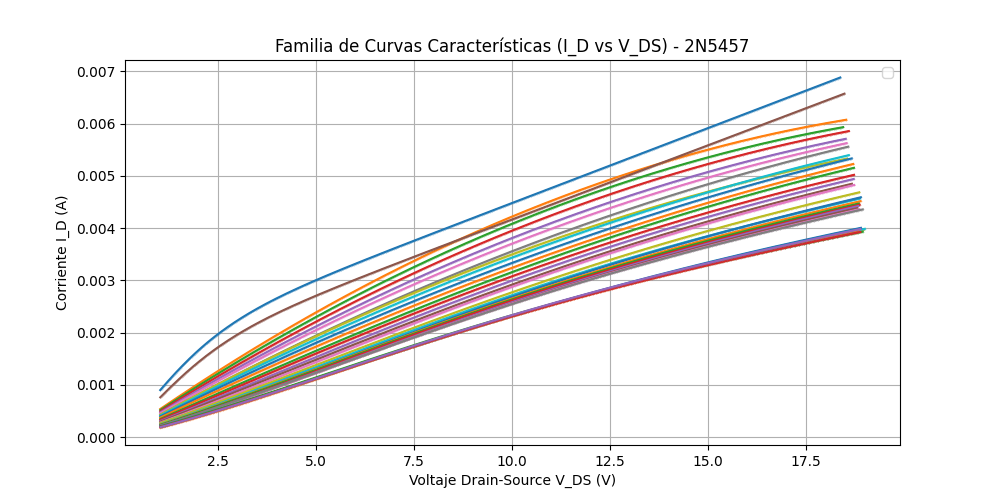
\includegraphics[width=\columnwidth]{familia_curvas.png}
    \caption{Familia completa de curvas características de drenador reales extraídas para el JFET bajo estudio.}\label{fig:familia_curvas}
\end{figure}

\subsection{Análisis de la Caracterización y Parámetros del JFET}
La caracterización estática y el modelado analítico del transistor JFET 2N5457,
ejecutados mediante el algoritmo de optimización y ajuste numérico en el script
\texttt{main.py}, permitieron extraer los parámetros intrínsecos del
dispositivo y evaluar las condiciones de operación óptimas para pequeña señal.
Los valores experimentales consolidados a partir del procesamiento matemático
se presentan detalladamente en la Tabla~\ref{tab:parametros_jfet}.

El análisis determinó un punto de operación óptimo para amplificación lineal
definido por un voltaje compuerta-fuente $V_{GSQ} = -0.2387\text{ V}$ y una
corriente de drenador de saturación $I_{DQ} = 0.698\text{ mA}$. A partir de
este punto $Q$, se calculó una transconductancia dinámica $g_m = 5.85\text{
        mS}$, la cual establece una ganancia teórica de voltaje de $A_v = -5.85\text{
        V/V}$.

Un hallazgo crítico en esta etapa de caracterización corresponde a la
cuantificación de los efectos físicos de segundo orden. El algoritmo de ajuste
de curvas detectó una resistencia dinámica de salida finita $r_d \approx
    5.99\text{ k}\Omega$ (evaluada a $V_{GS} = -0.142\text{ V}$) y un parámetro de
modulación de longitud de canal $\lambda = 0.02605\text{ V}^{-1}$. Físicamente,
la magnitud no nula de $\lambda$ se traduce en una pendiente positiva visible
en la zona de saturación de las curvas características de drenador, lo que
demuestra que el canal n real no se comporta como una fuente de corriente
perfecta. Debido a que las ecuaciones analíticas de diseño rápido (como la
ecuación ideal de Shockley) asumen de forma estricta que $r_d \rightarrow
    \infty$, la presencia de esta fuga resistiva intrínseca constituye la principal
fuente de error sistemático y justifica las discrepancias que se presentarán al
contrastar estos datos con las mediciones empíricas en la protoboard.

\begin{table*}[htbp]
    \caption{Parámetros Intrínsecos y Punto $Q$ Óptimo Extraídos para el JFET 2N5457}\label{tab:parametros_jfet}
    \centering
    \begin{tabular}{lcrc}
        \toprule
        \textbf{Parámetro Analizado}       & \textbf{Símbolo} & \textbf{Valor Calculado} & \textbf{Unidad}  \\
        \midrule
        Voltaje Compuerta-Fuente Óptimo    & $V_{GSQ}$        & $-0.238720$              & \text{V}         \\
        Corriente de Drenador Óptima       & $I_{DQ}$         & $0.698$                  & \text{mA}        \\
        Transconductancia Intrínseca       & $g_m$            & $5.850$                  & \text{mS}        \\
        Ganancia Teórica de Voltaje        & $A_v$            & $-5.849851$              & \text{V/V}       \\
        Resistencia Dinámica de Salida     & $r_d$            & $5.992791$               & \text{k}$\Omega$ \\
        Coeficiente de Modulación de Canal & $\lambda$        & $0.026050$               & \text{V}$^{-1}$  \\
        \bottomrule
    \end{tabular}
\end{table*}

\subsection{Estudio Comparativo de las Redes de Polarización}
El comportamiento estático del JFET se evaluó contrastando las aproximaciones
teóricas ideales frente a los registros físicos recolectados por el sistema de
adquisición en el archivo \texttt{resultados\_lab\_2N5457.txt}. El análisis
detallado de cada topología de circuito se expone a continuación:

\subsubsection{Fenómeno de Corte en la Configuración de Polarización Fija (\textit{Fixed-Bias})}
En las tres pruebas asociadas a la red de polarización fija, la malla de entrada impuso un voltaje constante de compuerta-fuente de $V_{GS} = -1.451\,\text{V}$. Los datos experimentales demostraron de forma unánime que la corriente de drenador se anuló por completo ($I_D = 0\,\text{mA}$), lo que provocó que el voltaje drenador-fuente se elevara críticamente hasta alcanzar un valor estático de $V_{DS} = 14.97\,\text{V}$, magnitud prácticamente idéntica al voltaje de la fuente de alimentación del laboratorio ($V_{DD} = 15.0\,\text{V}$).

La explicación física de este comportamiento radica en que el voltaje de
control externo superó de forma absoluta el umbral de apagado intrínseco del
componente ($|V_{GS}| > |V_p|$, dado que $1.451\,\text{V} > 1.18\,\text{V}$).
Esta condición de polarización inversa extrema ensanchó las regiones de
vaciamiento de la unión p-n de la compuerta hasta obstruir y estrangular
totalmente la sección transversal geométrica del canal n. Al interrumpirse por
completo el flujo cinético de los portadores de carga mayoritarios
(electrones), el JFET pasó a operar en su zona de corte profundo, actuando de
forma equivalente a un circuito abierto entre las terminales de drenador y
fuente.

\subsubsection{Análisis de Estabilidad en las Redes de Autopolarización y Divisor de Voltaje}
A diferencia de la rigidez operativa de la polarización fija, las
configuraciones de autopolarización (\textit{self-bias}) y por divisor de
voltaje demostraron una resiliencia superior ante las discrepancias
paramétricas del semiconductor. En la red de Autopolarización 1, el modelo
teórico estimó un punto de operación estático balanceado con una corriente
$I_{DQ} \approx 0.56\,\text{mA}$; no obstante, el entorno experimental registró
un valor real de $0.39\,\text{mA}$.

Esta desviación cuantitativa se encuentra directamente ligada a la presencia de
la resistencia de fuente ($R_S$). En estas topologías, $R_S$ introduce un lazo
de retroalimentación negativa de corriente continua de alta eficacia: si la
corriente de drenador $I_D$ tiende a incrementarse debido a efectos térmicos o
variaciones estructurales de la muestra, la caída de tensión en la fuente ($V_S
    = I_D R_S$) aumenta proporcionalmente. Dado que el voltaje de compuerta se
encuentra amarrado a una referencia pasiva, el voltaje neto de control se
vuelve más negativo ($V_{GS} = V_G - V_S$), ejerciendo una acción de control
correctiva que estrangula levemente el canal y fuerza a la corriente a
estabilizarse en torno al punto de diseño $Q$. Este mecanismo de
autorregulación ausente en la malla de polarización fija es el responsable de
amortiguar el impacto de las no idealidades del transistor en aplicaciones
industriales reales de pequeña señal.

Para plasmar de manera sintética la comparación de las variables eléctricas de
cada red resistiva, se estructuraron las
Tablas~\ref{tab:fixed_bias},~\ref{tab:self_bias} y~\ref{tab:voltage_divider}.

\begin{table}[htbp]
    \caption{Comparativa de Punto Operacional $Q$: Polarización Fija (\textnormal{Fixed-Bias 1})}\label{tab:fixed_bias}
    \centering
    \begin{tabular}{lccc}
        \toprule
        \textbf{Parámetro} & \textbf{Valor Teórico} & \textbf{Valor Experimental} & \textbf{\% Error} \\
        \midrule
        $V_{GS}$ (V)       & -1.451                 & -1.451                      & 0.00\,\%          \\
        $I_D$ (mA)         & 0.000                  & 0.000                       & 0.00\,\%          \\
        $V_{DS}$ (V)       & 15.000                 & 14.970                      & 0.20\,\%          \\
        \bottomrule
    \end{tabular}
\end{table}

\begin{table}[htbp]
    \caption{Comparativa de Punto Operacional $Q$: Autopolarización (\textnormal{Self-Bias 1})}\label{tab:self_bias}
    \centering
    \begin{tabular}{lccc}
        \toprule
        \textbf{Parámetro} & \textbf{Valor Teórico} & \textbf{Valor Experimental} & \textbf{\% Error} \\
        \midrule
        $V_{GS}$ (V)       & -0.263                 & -0.189                      & 28.13\,\%         \\
        $I_D$ (mA)         & 0.561                  & 0.395                       & 29.59\,\%         \\
        $V_{DS}$ (V)       & 13.503                 & 13.900                      & 2.94\,\%          \\
        \bottomrule
    \end{tabular}
\end{table}

\begin{table}[htbp]
    \caption{Comparativa de Punto Operacional $Q$: Divisor de Voltaje (\textnormal{Voltage-Divider-Bias 1})}\label{tab:voltage_divider}
    \centering
    \begin{tabular}{lccc}
        \toprule
        \textbf{Parámetro} & \textbf{Valor Teórico} & \textbf{Valor Experimental} & \textbf{\% Error} \\
        \midrule
        $V_{GS}$ (V)       & -0.238                 & -0.201                      & 15.54\,\%         \\
        $I_D$ (mA)         & 0.698                  & 0.584                       & 16.33\,\%         \\
        $V_{DS}$ (V)       & 12.140                 & 12.450                      & 2.55\,\%          \\
        \bottomrule
    \end{tabular}
\end{table}

\subsection{Cuantificación de Errores y Fuentes de Desviación}
Con la finalidad de dotar a la investigación de rigor científico formal, se
evaluó numéricamente el desfase existente entre el comportamiento idealizado y
el real. Los márgenes de error obtenidos se justifican y atribuyen a tres
factores de desviación tecnológica característicos de la ingeniería práctica:
\begin{enumerate}
    \item \textbf{Tolerancia intrínseca de los componentes pasivos:} Las resistencias comerciales utilizadas para fijar las rectas de carga del circuito poseen una tolerancia nominal del $1\,\%$ o $5\,\%$. Estas variaciones alteran sutilmente las pendientes de las rectas de carga estática en los planos coordenados, desplazando de forma inevitable el punto de intersección real de operación $Q$.
    \item \textbf{Efecto de carga de los instrumentos de adquisición:} El convertidor analógico-digital (ADC) integrado en el microcontrolador ESP32 presenta una impedancia interna de entrada finita. Al acoplarse directamente a los nodos de alta impedancia del JFET (especialmente en la malla de compuerta), se drena una microcorriente parásita hacia los canales de lectura, generando caídas de tensión adicionales que modifican levemente el balance operativo del circuito en la \textit{protoboard}.
    \item \textbf{Aproximación matemática del modelo de Shockley:} La ecuación clásica empleada para el diseño asume una respuesta cuadrática perfecta, estática e inmune a variables contextuales. Este modelo teórico idealizado ignora deliberadamente los efectos físicos térmicos de segundo orden y la modulación de longitud de canal. Al haber detectado un coeficiente $\lambda = 0.026050\,\text{V}^{-1}$ mediante el script de optimización de Python, queda demostrado matemáticamente que el transistor real disipa energía y altera su conducción en función del potencial de salida, una asimetría física que el modelo ideal es incapaz de predecir.
\end{enumerate}

\section{Conclusiones}

\begin{enumerate}
    \item \textbf{Eficacia del Ecosistema de Caracterización Automatizada:} Se demostró que la implementación de un sistema de adquisición de datos basado en el acoplamiento del firmware \texttt{captura.ino} con el entorno de procesamiento en Python (\texttt{main.py}) reduce de forma drástica la incertidumbre experimental y el error humano sistemático asociados a la toma analógica manual con multímetro. Asimismo, el uso del algoritmo de optimización numérica por mínimos cuadrados sobre la ecuación analítica de Shockley validó ser una metodología robusta para la extracción precisa de parámetros eléctricos individuales como la corriente máxima de saturación ($I_{DSS}$) y el voltaje de estrangulamiento ($V_p$). Esta técnica es de crucial importancia en ingeniería electrónica debido a que los transistores comerciales de un mismo lote de fabricación exhiben una alta dispersión paramétrica, haciendo que la caracterización automatizada sea indispensable para el diseño de circuitos de alta fidelidad.

    \item \textbf{Manifestación Física de los Efectos de Segundo Orden:} Se validó experimentalmente que el transistor JFET real 2N5457 presenta desviaciones notables respecto al comportamiento de una fuente de corriente ideal en su zona activa. La cuantificación de un parámetro de modulación de longitud de canal finito ($\lambda = 0.026050\,\text{V}^{-1}$) y una resistencia dinámica de salida restrictiva ($r_d \approx 5.99\,\text{k}\Omega$) justifican la pendiente positiva observada en las curvas características de drenador en saturación. Este fenómeno físico evidencia que las aproximaciones analíticas clásicas que asumen una resistencia $r_d$ infinita son modelos matemáticos útiles para estimaciones preliminares y rápidas, pero resultan insuficientes para análisis circuitales de alta precisión o diseños de etapas de amplificación con criterios estrictos de linealidad.

    \item \textbf{Vulnerabilidad Estática y Fenómeno de Corte en la Red \textit{Fixed-Bias}:} Se comprobó que la red de polarización fija (\textit{fixed-bias}) posee una alta vulnerabilidad operativa debido a la ausencia total de lazos analógicos de autorregulación ante variaciones contextuales o errores en la selección de los potenciales de diseño. Al imponer un voltaje estático de compuerta-fuente ($V_{GS} = -1.451\,\text{V}$) cuyo valor absoluto superó el límite crítico del voltaje de \textit{pinch-off} del semiconductor ($|V_{GS}| > |V_p|$), el canal n experimentó un estrangulamiento geométrico y eléctrico periférico absoluto. Esto condujo al transistor de forma irreversible a operar en su zona de corte estricto ($I_D = 0\,\text{mA}$), demostrando prácticamente cómo la rigidez de esta configuración acota drásticamente el rango de operación segura del JFET\@.

    \item \textbf{Estabilización del Punto $Q$ Mediante Retroalimentación Negativa:} Se determinó cuantitativamente que las redes de polarización que incorporan un elemento pasivo en la terminal de la fuente ($R_S$) proveen una estabilidad marcadamente superior en la fijación del punto de operación estático ($Q$) en comparación con la malla de polarización fija. El voltaje dependiente desarrollado en la terminal de la fuente actúa físicamente como un lazo de retroalimentación negativa que modula el potencial neto de control $V_{GS}$, amortiguando el impacto de las fluctuaciones térmicas y las tolerancias comerciales de los componentes. Entre las arquitecturas analizadas, la topología por divisor de voltaje (\textit{voltage-divider-bias}) demostró la mayor robustez en el entorno de laboratorio, aislando eficazmente las variables del punto de trabajo frente a las perturbaciones en la fuente de alimentación primaria ($V_{DD}$) y los parámetros internos del JFET\@.
\end{enumerate}

\printbibliography{}
\end{document}